\chapter{研究背景}
\label{chap:webapi}

本章では本研究の背景を、拡張現実についてのユーザーのデザイン要件に関する事前調査・分析と、拡張現実の普及との二点に分けて述べる。

\section{拡張現実について調査}
所属や肩書き関係なく20〜60歳の男女27人に対するインタビューを通してどのような拡張現実を望んでいるかのアンケートを集めた。その結果からどのようなデザイン要件が求められているのかを明確にする。

\subsection{拡張現実を体験するために一般的な人々が支払う金額}
機能性やデザインの詳細を伝えた上で、仮想現実を見る手段として次の選択肢の中から選んでもらった。OCULOUS Rift:85278円、ハコスコ:1500円、iWink:36478円、タカラトミー夢工房:15984円、DreamScape :無料。図はその結果である。

\begin{figure}[htbp]
\begin{center}
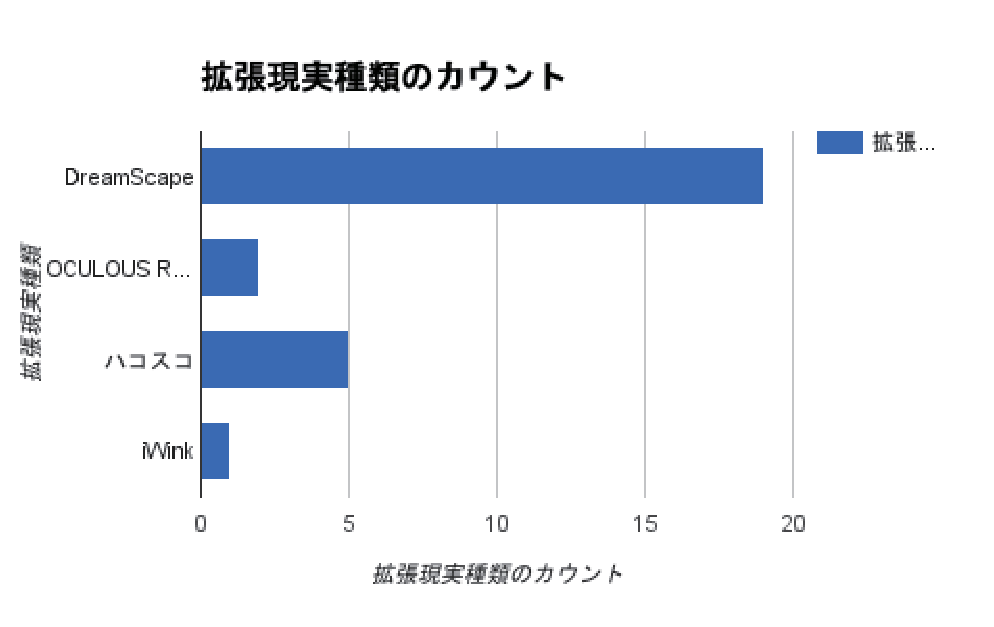
\includegraphics[width=15cm]{eps/VRselection.eps}
\caption{拡張現実を体験するために一般的ユーザーが選ぶ手段}
\label{拡張現実を体験するために一般的ユーザーが選ぶ手段}
\end{center}
\end{figure}

一般的なユーザーの中には拡張現実を体験するためにOCULOUS Riftあどの高額なデバイスを購入しようとする人は少ないということが分かった。ハコスコだと少し人数が増える。これらのデータから無料で簡単に手に入れることができるツールは必要とされているということが分かった。

\subsection{拡張現実を体験したいタイミング}
拡張現実を体験したいタイミングとして、睡眠中と起きている時間帯でどちらが好ましいかについて調査を行った。すると図のようにあまり差がなかった。睡眠中と回答した人の理由としてあげていたのは睡眠時間の有効活用っであった。比べて起きている時と答えた人は起きたら忘れてしまうかもしれないから、意識のある時に体験したいと答えた。よってDreamScapeの開発で実際に睡眠中の拡張現実がユーザーにどのような体験を与えるのかを研究する意義があると考えられる。

\begin{figure}[htbp]
\begin{center}
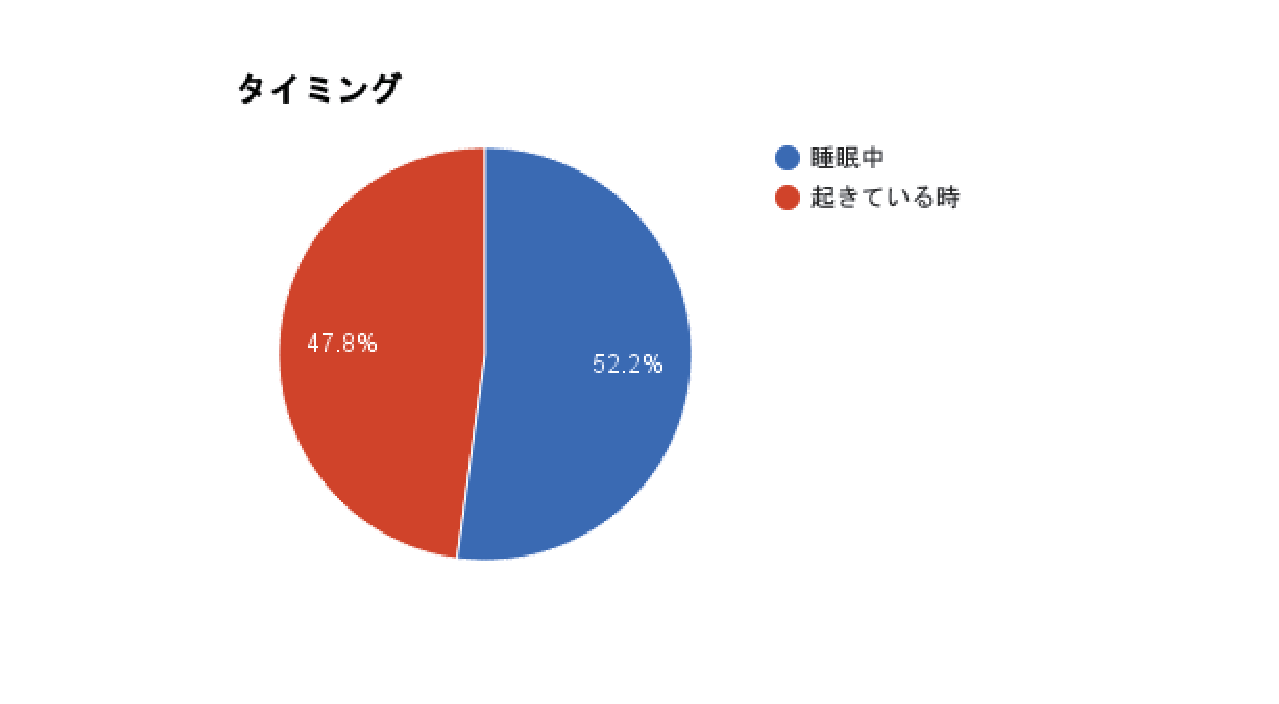
\includegraphics[width=15cm]{eps/timing.eps}
\caption{拡張現実を体験したいタイミング}
\label{拡張現実を体験したいタイミング}
\end{center}
\end{figure}

\section{明晰夢に関する調査}
\subsection{夢をどのくらい記憶しているか}
夢の操作に成功したとしてもその夢を覚えていなければ意味がない。そこで実験を始める前に一般的に人は夢の内容を起床後どのくらい覚えているのかを調査した。図がから読み取れるように、夢を置く覚えていると答えた人は少数だった。
\begin{figure}[htbp]
\begin{center}
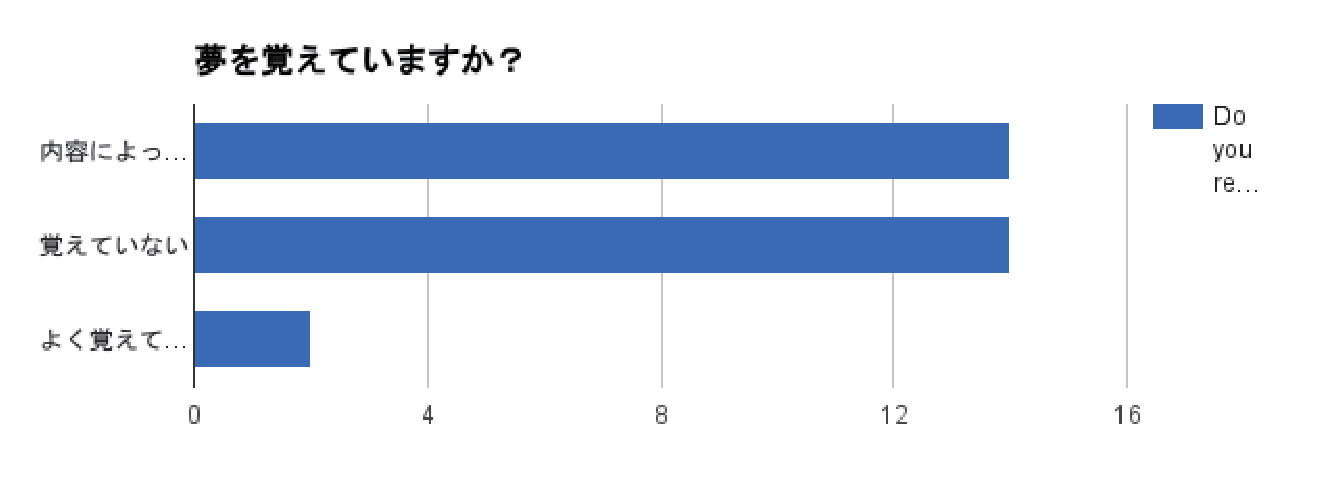
\includegraphics[width=15cm]{eps/remember.eps}
\caption{拡張現実を体験したいタイミング}
\label{拡張現実を体験したいタイミング}
\end{center}
\end{figure}
覚えている夢は刺激的、怖い夢、繰り返し見た夢というのが多く、日常的な夢は忘れがちであるということが分かった。人は夢の90\%を起床後5分間で忘れるという。夢を忘れないためによく取られる手法は夢日記である。よってDreamScapeには5分以内に夢の内容を記憶するための日記の機能を加えることに決めた。夢日記は習慣的につけることで効果が出ると言われている。なのでDreamScapeの実験に参加してもらう人には2週間前から枕の横に紙とペンを置いて起床後すぐに夢の内容を書いてもらう習慣をつけてもらうことにした。

\subsection{夢に影響を与えやすい外的刺激}
心理学者フロイトは「夢判断」の中で人は睡眠中の姿勢、環境、身体的刺激によって夢の内容が変化すると言っている\cite{freud}。\\
睡眠中の人間の鼻先を羽毛でくすぐったときに、夢の内容に変化があったことを確認する実験を紹介している。そこで音、体制、匂い、振動、光、などの刺激の中で何が夢に一番影響を与えやすいのかの調査をした。以下の図がその結果を示す。
\begin{figure}[htbp]
\begin{center}
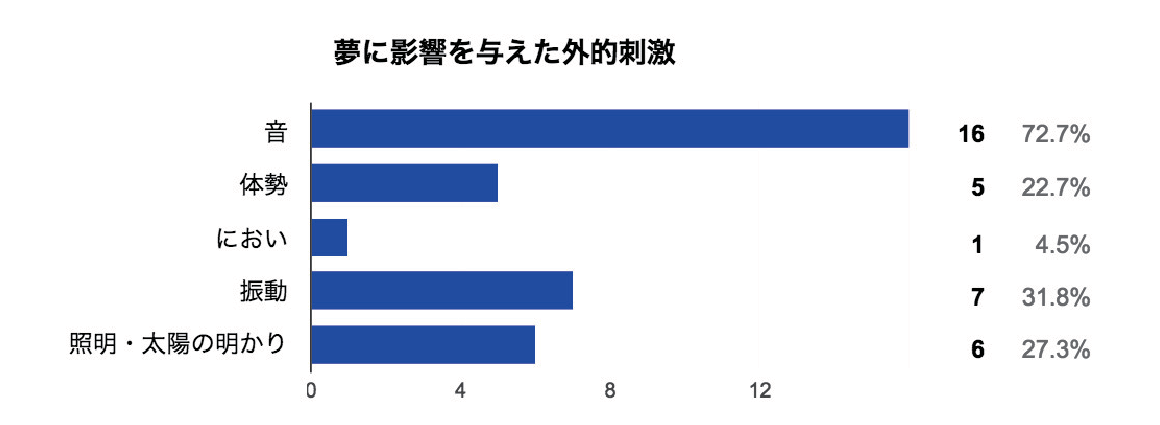
\includegraphics[width=15cm]{eps/input.eps}
\caption{夢に影響を与えた外的刺激}
\label{夢に影響を与えた外的刺激}
\end{center}
\end{figure}
音が他の刺激よりも影響を与えやすいということが分かった。DreamScapeにとって刺激は非常に重要な鍵となるので実験を通してどの刺激が最も有効的なのかを調べた。それについて第3章を参照してほしい。

\subsection{明晰夢のニーズ}
明晰夢を体験したいか否かで質問をしたところ、77%の人が体験したいと答えた。以下がその図である。よってDreamScapeのニーズもあると仮定する。
\begin{figure}[htbp]
\begin{center}
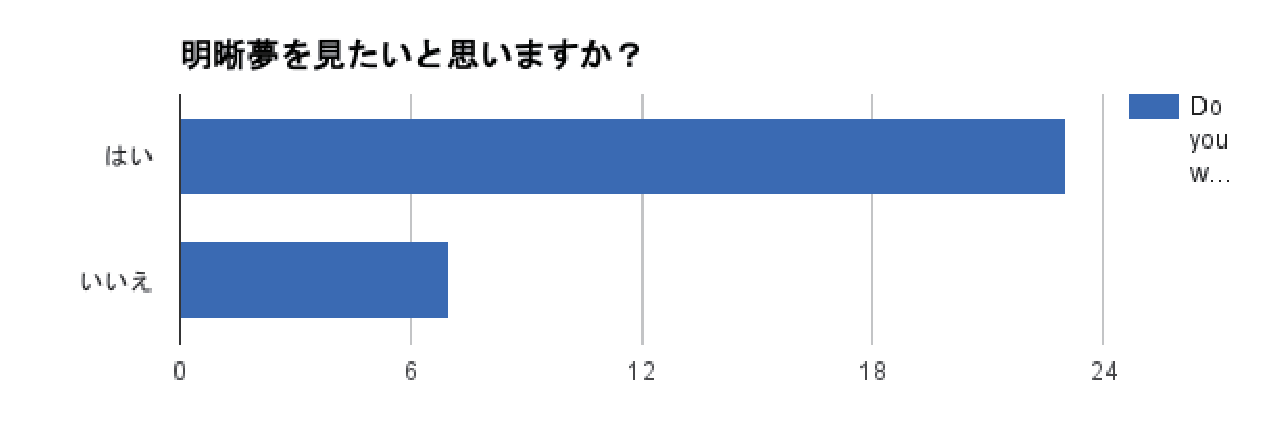
\includegraphics[width=15cm]{eps/lucidDreamingYesNo.eps}
\caption{明晰夢のニーズ}
\label{明晰夢のニーズ}
\end{center}
\end{figure}

\subsection{明晰夢で体験したい内容}
拡張現実で体験したい内容で多かったのは以下の図で確認でききる。LOVEタイプとは恋愛や性的行為などが含まれる内容の物。アドベンチャータイプは冒険など非日常の体験を求める物。ストリータイプはドラマのように連続性のある夢をみることをいう。癒しタイプ・元気欲しいタイプは娯楽を求める夢。現実的タイプで少数派としてエロいタイプと勉強家タイプがあった。
\begin{figure}[htbp]
\begin{center}
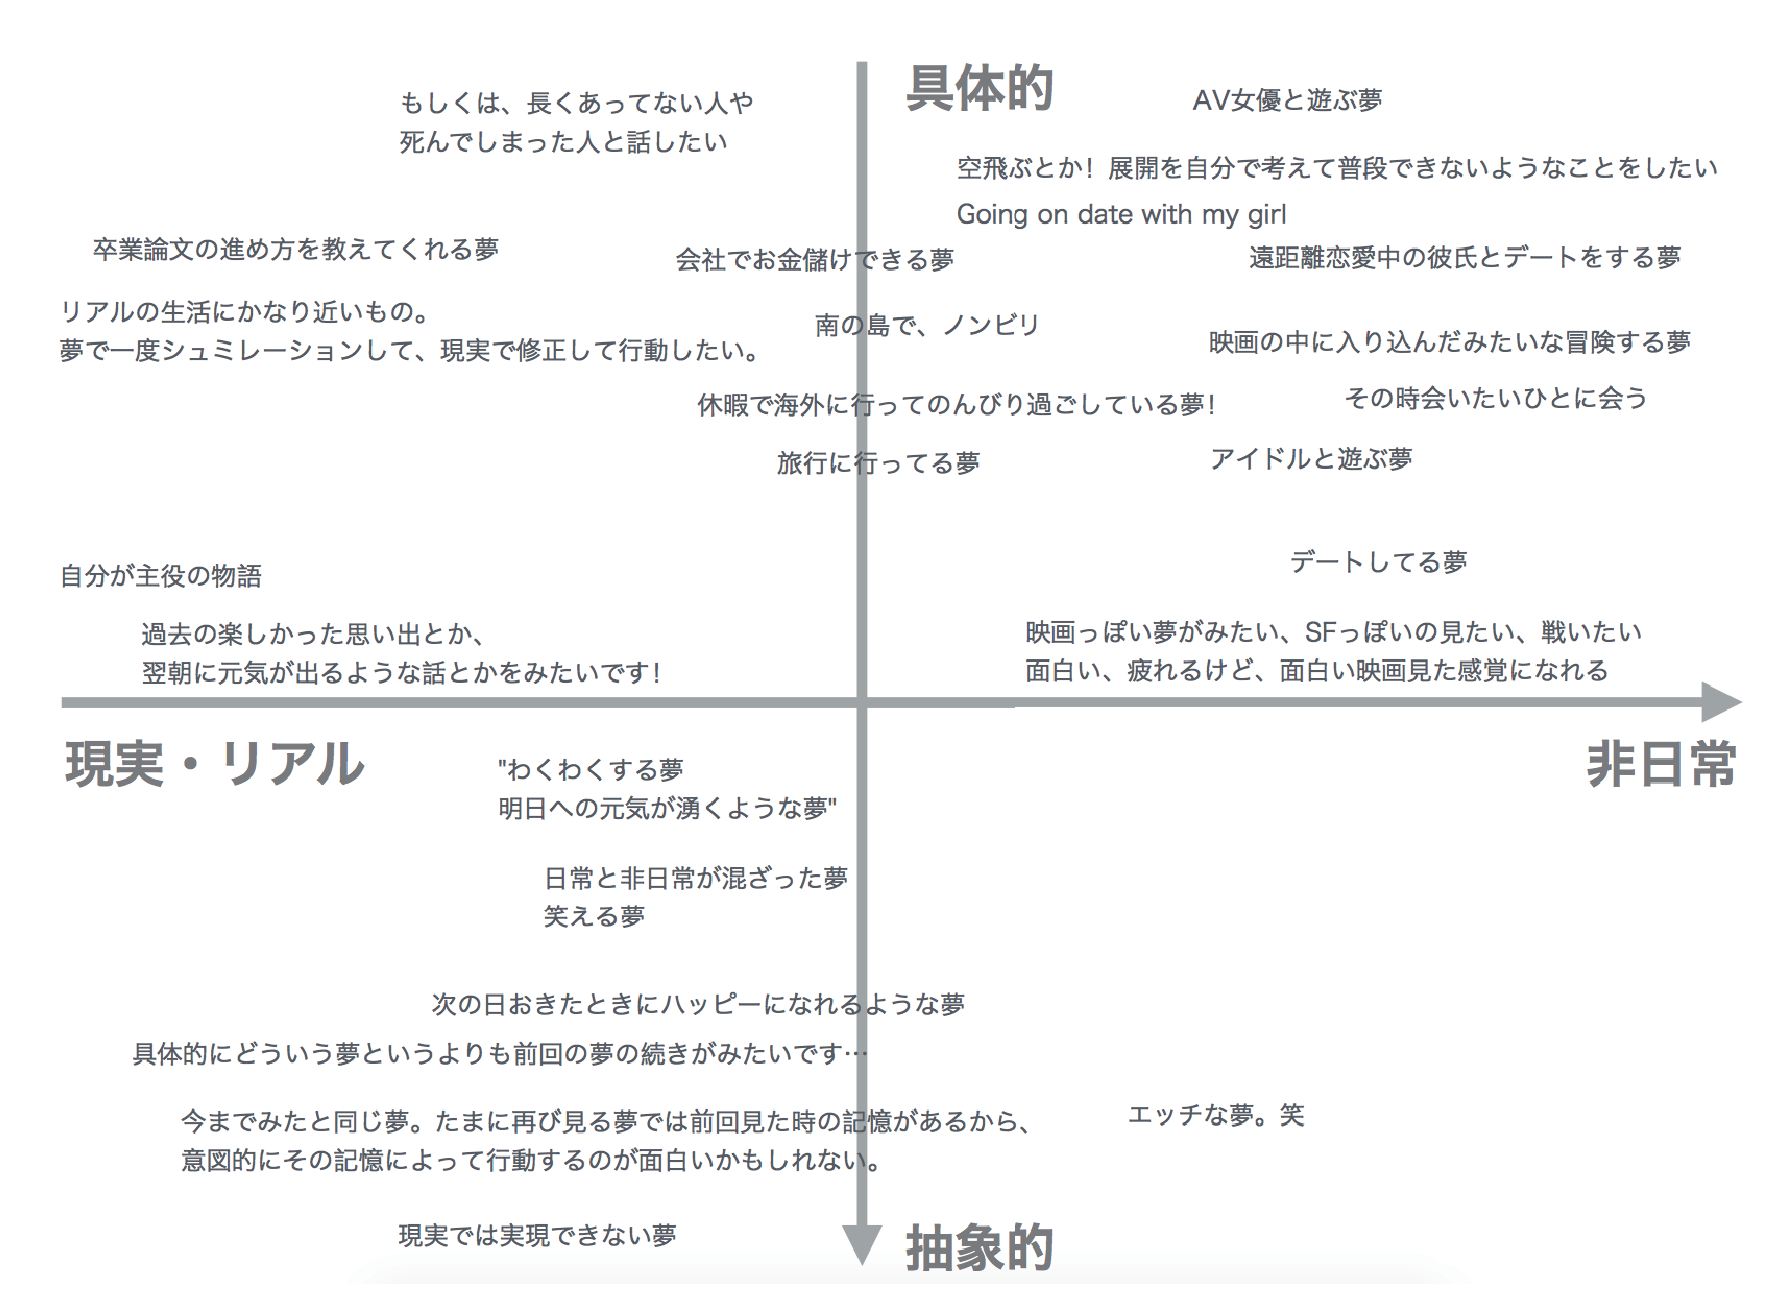
\includegraphics[width=15cm]{eps/whatYouWantToDream.eps}
\caption{明晰夢で体験したい内容:分析1}
\label{明晰夢で体験したい内容:分析1}
\end{center}
\end{figure}

\begin{figure}[htbp]
\begin{center}
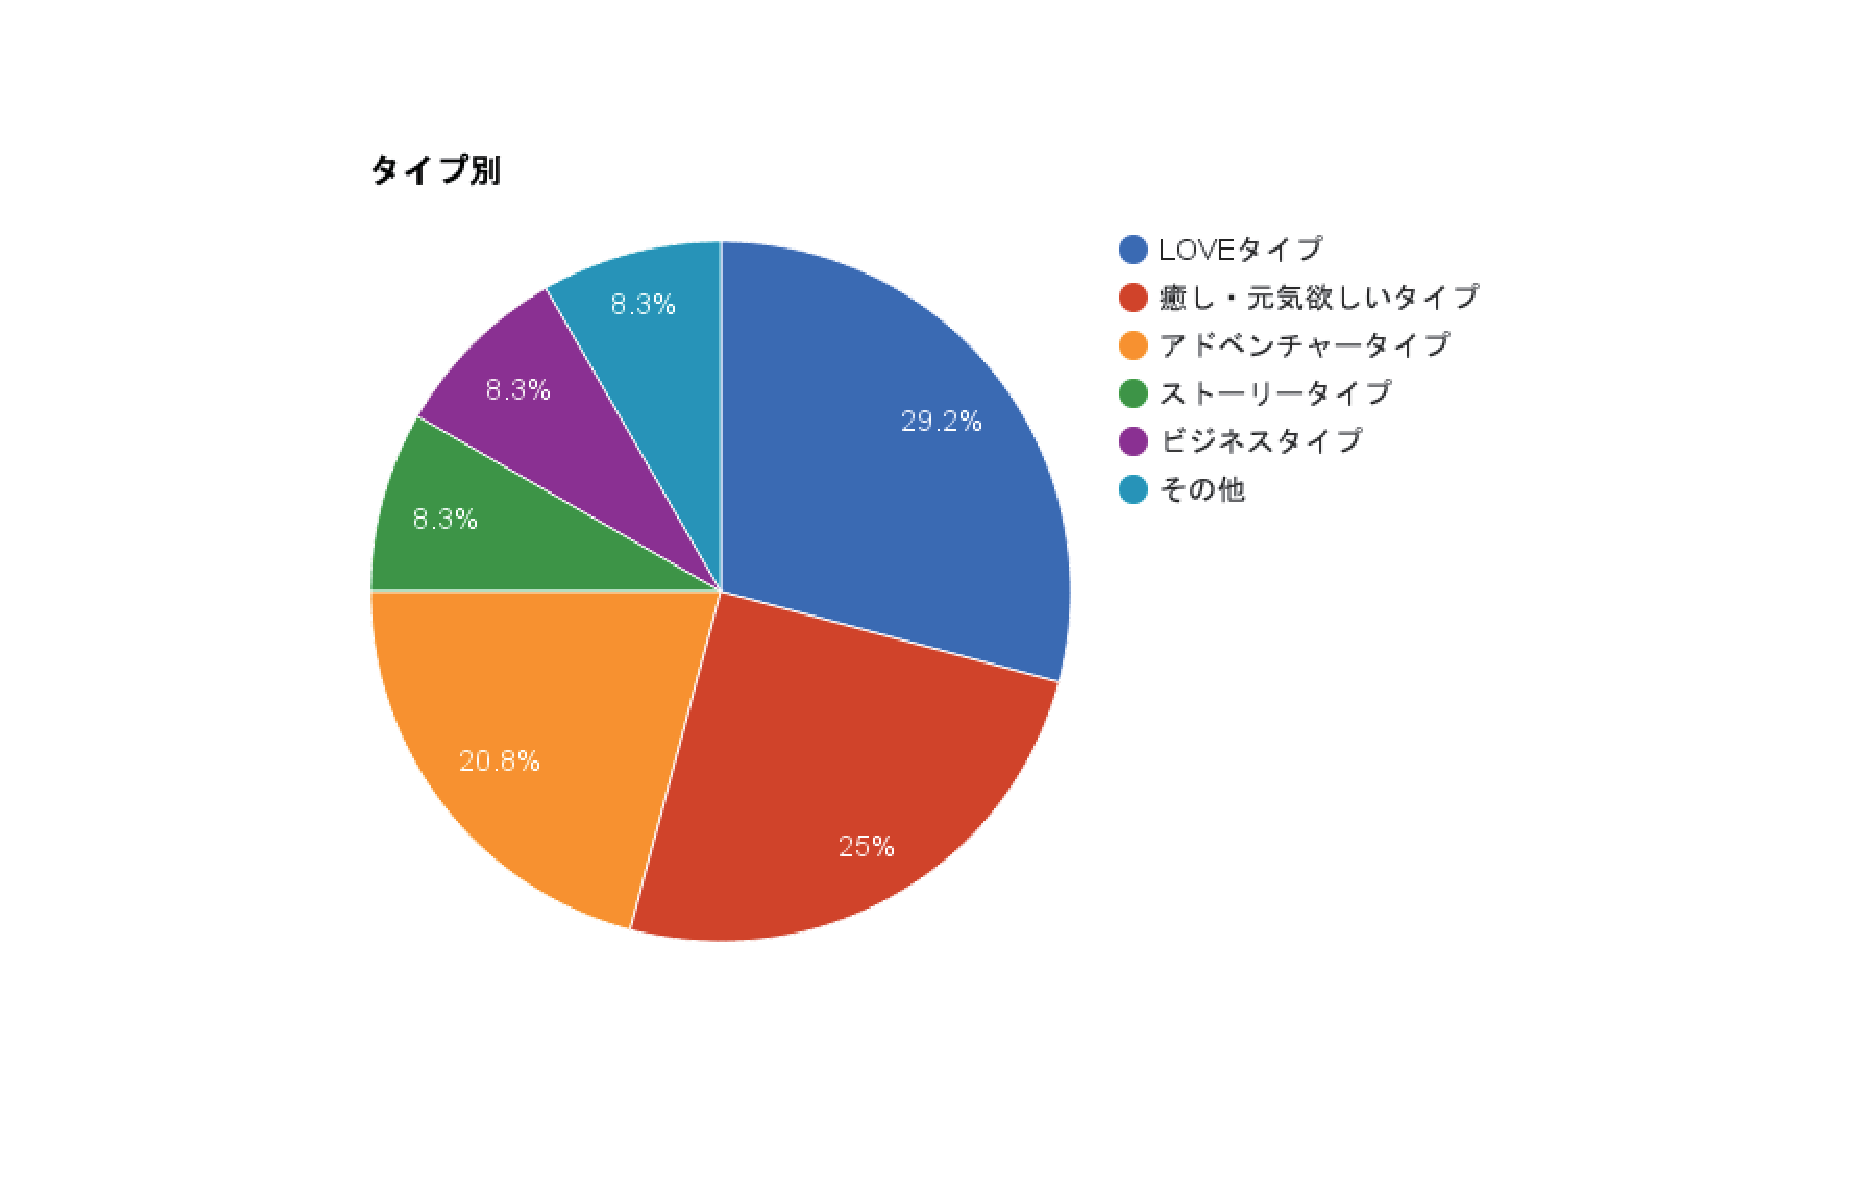
\includegraphics[width=15cm]{eps/dreamType.eps}
\caption{明晰夢で体験したい内容:分析2}
\label{明晰夢で体験したい内容:分析2}
\end{center}
\end{figure}

\section{拡張現実体験する手段として主流の手段とされているVirtual Realityではなく明晰夢に着目した背景}
 拡張現実を体験したがっている。昨今ではVRが注目されているが、現実を仮想的に見るのは明晰夢という形でも可能なのであれば興味のある人も多い。VRは様々なツールが必要とされ、金銭的コストがかかってしまう。比べて明晰夢は全ての人間が行う睡眠という習慣をより有効に活用し、金銭的コストをかけることなく遂行することができるのである。求められるのは、値段、機能性、デザインなのでその点に気をつけて開発を進めたい。また、コンテンツが見られるようにする対策も必要である。

%\subsection{テレイグジスタンスについて}
%昨今ではVirtual Reality( VR)が活発に研究されるようになった。 VR とはコンピューターにより趣味レーションされた拡張現実を見せて、ユーザーがインタラクションできるようにすることである。Virtual Reality最大の試練はその拡張現実をより現実的に感じさせるために、映像の見せ方、インタラクションの行われ方、音の聞こえ方を追求することされてきた\cite{vrtrendShiny}。\\
% VRの中でもテレイグジスタンスという分野では、各地にあるものや人ががあたかも近くにいるかのように感じながら、操作などをリアルタイムに行う環境を構築する技術および体型のことで、慶應義塾大学 大学院メディアデザイン研究科の舘\UTF{66B2}教授によって1984年に初めて紹介された。引用
%使用例1:人間が行く事が困難な場所での危険作業が出来るものとして期待されている。使用例2:火星、金星開発も人間が直接行って開発するのではなく、地球にいながらテレイグジスタンスの技術を使って開発すえる
%\subsection{明晰夢について}
%明晰夢に対して:本研究の中では、明晰夢という定義としてPaul Thoelyの記した定義を流用する。REM睡眠中に起こる現象引用Paul Thoelyは以下は明晰夢を以下の条件全てが一致したときにのみ、明晰夢と断定することとしている。(1)夢を見ているということを自覚する。(2)夢において自覚的に判断を行う。(3)起床後も夢に関する記憶がある。(4)夢においての自分の存在を理解する(5)夢の中で自分が置かれている環境を理解する(6)夢の意味を理解する(7)集中度を自覚する。明晰夢の経験者はしばしば、夢の状況を自分の思い通りに変化させられると語っている。このスキルを獲得するには時間と労力が必要とされてきた。哲学者や心理学者により研究が重ねられてきた。娯楽やセラピーで使われている。明晰夢利用例1引用(英語の論文)
%\section{現状のまとめと問題の分析}
%(ターゲット・明晰夢を手段として選ぶ理由・デザイン要件)
%昨今ではVRが注目されているが、現実を仮想的に見るのは明晰夢という形でも行われてきた。VRと明晰夢の違いを下記の図で詳しく述べる。図(金銭的コスト・時間的コスト・配布しやすさ・開発度・使われ方・分野)(1P)。VRは様々なツールが必要とされ、金銭的コストがかかってしまう。比べて明晰夢は全ての人間が行う睡眠という習慣をより有効に活用し、金銭的コストをかけることなく遂行することができるのである。

%WebAPIとは、インターネットを介して利用することのできるアプリケーション・プログラミング・インターフェイス(API)のことである。殆どのWebAPIが一般的なURLの形式を取っており、HTTPによるPOSTメソッドを用いて、パラメータを付加したURLを使用してアクセスしてデータを取得する。返ってくるデータはXML、JSONのどちらかが一般的である。今回用いるWebAPIは、以下の4つである。

%\subsection[Yahoo!検索Web API-ウェブ検索API]{Yahoo!検索Web API-ウェブ検索API\protect\footnote{ウェブ検索APIは、2013年3月頃を目処にAPIのリクエストURLが変更される予定であり、これはそれまで公開されていたアップグレード版ウェブ検索APIを使用している。}}
%\begin{table}[htdp]
%\begin{tabular}{c|l}
%開発 & ヤフー株式会社 \\
%URL & http://search.yahooapis.jp/PremiumWebSearchService/V1/webSearch \\
%機能 & Web上に公開されているページを検索する
%\end{tabular}
%\end{table}
%\subsection[Yahoo!検索Web API-画像検索API]{Yahoo!検索Web API-画像検索API\protect\footnote{画像検索APIは、2013年3月頃を目処にAPIのリクエストURLが変更される予定であり、これはそれまで公開されていたアップグレード版画像検索APIを使用している。}}
%\begin{table}[htdp]
%\begin{tabular}{c|l}
%開発 & ヤフー株式会社 \\
%URL & http://search.yahooapis.jp/PremiumImageSearchService/V1/imageSearch \\
%機能 & Web上に公開されている画像を検索する
%\end{tabular}
%\end{table}
%\subsection{Youtube Data API}
%\begin{table}[htdp]
%\begin{tabular}{c|l}
%開発 & Google Inc. \\
%URL & http://gdata.youtube.com/feeds/api/videos \\
%機能 & Youtubeの機能(動画の検索、アップロード、再生リストの作成など)を利用する
%\end{tabular}
%\end{table}
%\subsection{Product Advertising API}
%\begin{table}[htdp]
%\begin{tabular}{c|l}
%開発 & Amazon.com, Inc.\\
%URL & http://ecs.amazonaws.jp/onca/xml \\
%機能 & Amazon の商品情報や関連コンテンツを検索する
%\end{tabular}
%\end{table}